% mnras
% \documentclass[fleqn,useAMS,usenatbib]{mnras}

% apj
%\documentclass[iop, twocolappendix, appendixfloats, numberedappendix, apj]{emulateapj}
\documentclass[iop, twocolappendix, appendixfloats, numberedappendix, apj]{hackemulateapj}
%\documentclass{emulateapj}

%=====================================================================
% CUSTOM: PACKAGES, MACROS & SETTINGS
%=====================================================================
% packages for figures
\usepackage{graphicx,todonotes}

% packages for symbols
\usepackage{latexsym,amssymb}

% AMS-LaTeX package for e.g. subequations
\usepackage{amsmath,morefloats}
\usepackage[backref,breaklinks,colorlinks,citecolor=blue]{hyperref}
\usepackage{natbib,graphicx,amsmath,subfigure,color,xcolor}
%\usepackage{natbib,graphicx,amsmath,subfigure,color,xcolor,hyperref}
\usepackage{verbatim}
\usepackage{threeparttable}

\usepackage{pgfplots}
\pgfplotsset{compat=newest}
\usepgfplotslibrary{fillbetween}
\usepgfplotslibrary{groupplots}


%\usepackage{lineno}
%\linenumbers

\topmargin-1cm

\newcommand\notedo[1]{\todo[color=yellow, inline, size=\small]{To do:#1}}
\newcommand\notewrite[1]{\todo[color=orange, inline, size=\small]{To write: #1}}
\newcommand\noteask[1]{\todo[color=cyan, inline, size=\small]{To ask: #1}}
\newcommand\notecontrib[1]{\todo[color=green, inline, size=\small]{Contributors: #1}}
\newcommand{\mattodo}[1]{\textcolor{red}{[MRB TODO: \bf #1]}}
\newcommand{\esstodo}[1]{\textcolor{orange}{[ESS TODO: \bf #1]}}
\newcommand{\ess}[1]{\textcolor{blue}{[ESS: \bf #1]}}
\newcommand{\mrb}[1]{\textcolor{purple}{[MRB: \bf #1]}}

\newcommand{\descwl}{\texttt{WeakLensingDeblending}}

\newcommand{\vecg}{\mbox{\boldmath $g$}}
\newcommand{\vece}{\mbox{\boldmath $e$}}
\newcommand{\veck}{\mbox{\boldmath $k$}}
\newcommand{\vecQ}{\mbox{\boldmath $Q$}}
\newcommand{\vecF}{\mbox{\boldmath $F$}}
\newcommand{\vecD}{\mbox{\boldmath $D$}}
\newcommand{\vecc}{\mbox{\boldmath $c$}}
\newcommand{\vecm}{\mbox{\boldmath $m$}}
\newcommand{\matR}{\mbox{$\bf R$}}
\newcommand{\matC}{\mbox{$\bf C$}}
\newcommand{\bnab}{\boldsymbol{\nabla}}
\newcommand{\bnabg}{\boldsymbol{\nabla_g}}
\newcommand{\galsim}{\texttt{GALSIM}}
\newcommand{\ngmix}{\texttt{ngmix}}
\newcommand{\nnsim}{\texttt{nsim}}
\newcommand{\snr}{$S/N$}
\newcommand{\sn}{$S/N$}
\newcommand{\coadd}{{\rm coadd}}
\newcommand{\desreq}{$4\times 10^{-3}$}
\newcommand{\lsstreq}{$2\times 10^{-3}$}

\newcommand{\calexp}{\texttt{Exposure}}
\newcommand{\dm}{\texttt{LSST DM}}

\newcommand{\mcal}{\textsc{metacalibration}}
\newcommand{\mdet}{\textsc{metadetection}}
\newcommand{\Mcalshort}{\textsc{metacal}}
\newcommand{\Mcal}{\textsc{Metacalibration}}
\newcommand{\Mdet}{\textsc{Metadetection}}
\newcommand{\vest}{\mbox{\boldmath $e$}}
\newcommand{\est}{e}
\newcommand{\mcalR}{\mbox{\boldmath $R$}}
\newcommand{\mcalRS}{\mbox{\boldmath $R_S$}}
\newcommand{\gest}{\mbox{\boldmath $\hat \gamma$}}
\newcommand{\vecgam}{\mbox{\boldmath $\gamma$}}

\newcommand{\sx}{\textsc{Source Extractor}}

\newcommand{\bfd}{\textsc{BFD}}

\newcommand{\vonkarman}{{von K\'arm\'an}~}


%\setuphead[section][before={\testpage[2]}]

%mnras
%\title[\Mdet]{\Mdet: Mitigating Shear-dependent Object Detection Biases with \Mcal}

%\author[Sheldon et~al.]{Erin Sheldon$^1$, Matthew R. Becker$^2$,
%Niall MacCrann$^{3,4}$, Michael Jarvis$^5$
%  \\$^1$Brookhaven National Laboratory, Bldg. 510, Upton, NY 11973, USA
%  \\$^2$High Energy Physics Division, Argonne National Laboratory, Lemont, IL 60439, USA
%  \\$^3$Center for Cosmology and Astro-Particle Physics, The Ohio State University, Columbus, OH 43210, USA
%  \\$^4$Department of Physics, The Ohio State University, Columbus, OH 43210, USA
%  \\$^5$Department of Physics and Astronomy, University of Pennsylvania, Philadelphia, PA 19104, USA
%}


% apj
\shorttitle{Metadetection for Rubin}
\shortauthors{Sheldon, Becker, Armstrong}

\begin{document}
% mnrad
% \date{Draft \today}

% mnras
%\maketitle


% apj
%\title{\Mdet: Mitigating Shear-dependent Object Detection Biases with \Mcal}
\title{Metadetection for the Vera C. Rubin Observatory}

\author{Erin S. Sheldon}
\affil{Brookhaven National Laboratory, Bldg 510, Upton, New York 11973, USA}
\author{Matthew R. Becker}
\affil{High Energy Physics Division, Argonne National Laboratory, Lemont, IL 60439, USA}
\author{Michael Jarvis}
\affil{Department of Physics and Astronomy, University of Pennsylvania, Philadelphia, PA 19104, USA}
\author{Robert Armstrong}
\affil{Lawrence Livermore National Laboratory, Livermore, CA 94551, USA}


\begin{abstract}

    \Mcal\ for LSST

\end{abstract}

% \newpage
% \tableofcontents

\section{Introduction} \label{sec:intro}

\esstodo{}

\section{Simulation Features} \label{sec:sim}

We simulated what are known in the LSST data management system (\dm, TODO cite)
as calibrated exposure images.  This data is stored in a data structure known
as as a \calexp, which carries with it the calibrated, background subtracted
image data, along with an estimated noise variance image plane, world
coordinate system transformation (WCS) and position dependent PSF model.
Problem areas associated with saturation, cosmic rays, and bad columns are
marked in an integer big mask image plane.

We stored the true values for all these data in the \calexp\ data structure
passed onto the measurement algorithms, with the exception of the background
which was optionally offset in order to test re-estimation of the
background on the coadd.

The basic simulation was similar to that created for the \mdet\ \citep{mdet20} and
DES \mdet\ papers (TODO cite DES mdet test paper).  All images were rendered
using the \galsim\ python package (TODO cite galsim).  In the following
sections we describe each of the image features.

For this work, we used the simulation package \texttt{descwl-shear-sims}
version 0.4.0\footnote{\url{https://github.com/LSSTDESC/descwl-shear-sims}}.

\subsection{Image Filters and Noise} \label{sec:sim:noise}

We used the \descwl\ package (TODO cite) to determine the
noise for images in each filter.  In all simulation runs we used predicted
noise $n$ for the final 10 year coadd.  For individual simulated epochs we
re-scale the noise appropriately, such that the noise in each epoch was $n *
\sqrt{N}$.  We used a Guassian random field to simulate the noise, which is a
good approximation at the expected noise levels (TODO cite).

We did not add the expected amount of background to each image (but see \S
\ref{sec:sim:bgerr}).  After drawing all image features and adding
noise, we re-scaled the images to a common zero point of 30.

\subsection{Image World Coordinate System, Rotations and Dithers} \label{sec:sim:rotdith}

Each image was simulated as a tangent plane projection of the sky onto the
image frame with the LSST camera pixel scale of 0.2 arcseconds (TODO reference).
The world coordinate system (WCS) transformation between sky and pixel
coordinates was represented as a \galsim\ \texttt{TanWCS} object.  Each
simulated WCS transformation had a random rotation applied, in order to mock up
the camera rotations used by LSST cam (TODO cite proper paper).  The center of
each image was shifted, or ``dithered'', randomly in two dimensions relative to
the center of the desired coadded image.  We choose the dithers to be a
unrealistically small, within two pixels, to minimize portions of the image
that would not overlap the final coadd.  The image size was just large enough
so that the rotated image, after dithers, would have no edge crossing the coadd
region, again to avoid waste:  coadding an image with an edge produces a
discontinuous PSF in the final coadd, so such images would be discarded.

\subsection{Point Spread Function} \label{sec:sim:psfs}

\mattodo{Briefly describe PS PSF and link to original mdet paper and possibly
DES paper.}

\subsection{Stars} \label{sec:sim:stars}

We simulated stars using fluxes and densities sampled from the LSST DESC DC2
simulation (TODO cite).  For each simulated field we sampled randomly, with
replacement, from the map of stellar density used to generate DC2, with a
maximum allowed density of 100 per square arcminute.  This density represents
the total number of stars drawn, not the number detected.  To determine each
stars multiband flux, we sampled stars from the DC2 star catalog.  We modeled
each star as a small Gaussian (FWHM $= 10^{-4}$ arcsec) convolved with the
point spread function.  We drew stars at random locations, even when galaxies
were drawn on a grid layout (see \S \ref{sec:sim:layouts}).  Stars were allowed
to saturate and have an associated bleed trail (see
\S \ref{sec:sim:satbleeds}).

\subsection{Image Saturation, Star Masking and Star Bleed Trails} \label{sec:sim:satbleeds}

The value in each pixel was artificially limited in order to simulate
saturation, and saturated pixels were marked with the appropriate flag an
integer bitmask image, and set the variance is set to infinity.  Non linear
detector response was not simulated.

Saturated stars were over-drawn with a simulated bleed trail image, taken from
a set of previously generated templates.  The bleed templates were identified
in images of bright stars created using the DC2 code.  For each saturated star
in our simulation, we found a close template match in the filter of interest
and drew the associated bleed image directly over the star image with a value
set to the saturation level. The bleed pixels were marked with the appropriate
flag in the bitmask.

We marked saturated stars in the bitmask image with a circular mask that
covered the star out to the radius where the profile reached the noise level.
Note in real data such a mask would need to be determined algorithmically.
This mask does not necessarily cover the bleed trail completely, although the
trail was interpolated (see \S \ref{sec:coadding}).  We find that these
unmasked trails do not cause a shear bias, which we attribute to the
camera rotations, which randomize the direction of the trail on the sky.

\subsection{Cosmic Rays} \label{sec:sim:cosmics}

\mattodo{Briefly describe and link to DES paper, note affect on image and
bitmask/variance plane}

\subsection{Bad Columns} \label{sec:sim:badcols}

\mattodo{Briefly describe and link to DES paper, note affect on image and
bitmask/variance plane}

\subsection{Galaxies} \label{sec:sim:galaxies}

We used the \descwl\ package to generate galaxy models (TODO cite).  These
elliptical, color models have bulge, disk and AGN components. We performed the
drawing of these models in our code in order to enable the use of our on PSF
models (see \S \ref{sec:sim:psfs}, and to allow for more efficient drawing.

We also performed simulation runs with one component, round exponential
galaxies with fixed flux and size.  These models are useful for shear recovery
tests that do not require a realistic galaxy population, but benefit from using
low shape noise shear tracers.  These models were most often used as moderately
fast, full shear recovery tests, to further test code changes
that have already passed the fast unit tests.

\subsection{Layouts} \label{sec:sim:layouts}

We ran tests with both random and gridded galaxy layouts.  The random layout
was used with the realistic galaxy population, and the density of objects
reflected the expected density of galaxies as defined in the \descwl\ package.

The grid was used with the simple, round exponential galaxies to facilitate
moderately fast shear recovery tests.  The grid is square, with spacing
designed to avoid overlap between adjacent galaxies, and thus avoid blending
effects.

See \S \ref{sec:sim:galaxies} for descriptions of each galaxy model type.

\subsection{Image Background} \label{sec:sim:bgerr}

We add a negative constant to the images to approximate errors in the
background determination.  The motivation is to test if errors for individual
epochs can be corrected in the final coadd image by running a second background
determination (TODO reference a section where the result is mentioned).

\subsection{Shear Patterns} \label{sec:sim:shears}

We implemented two different types of shear pattern.  In one we used a single
shear for all images, with constant magnitude and orientation.  The second type
was a constant magnitude shear, but with random orientation for each image.
These two scenarios result in equivalent shear recovery bias when objects are
not divided into cells on the sky (see \S \ref{sec:sim:cells}) but, as we will
see in \S \ref{sec:results:randshear}, a small additional selection bias is
introduced for random shears when when trimming to cells.

\subsection{Overlapping Coadd Cells} \label{sec:sim:cells}

Coadds can be used for shear measurement (TODO cite bob's paper), but we
require that the coadded images have a continuous PSF in order to faciliate
accurate PSF modeling.  Images that have an edge in the coadd region must be
rejected.  Smaller coadds result in fewer images being rejected, but very small
coadds would complicate object identification deblending.  For LSST, we plan to
use relatively small (250x250 pixels) overlapping (50 pixels) coadded regions
for shear measurement, which we call ``cells'' (TODO cite).

We ran simulations with and without cells in order control for issues specific
to the cell processing and trimming of objects to non overlapping regions.  We
adopted the cell definitions outlined above: 250x250 pixel cells with 50 pixel
overlaps. The object list was trimmed to the non-overlapping region in post
processing.

\subsection{Noise Images} \label{sec:sim:noiseimages}

The \mcal\ procedure involves deconvolution by the PSF, shearing of the image,
and reconvolution by a round kernel.  This process alters the noise and
produces a spurious shear response.  We can cancel this bias by adding a noise
image, with properties that statistically match the real background noise,
processed in a similar manner but with orthogonal shear.  We stored this
noise image in a copy of the image \calexp\ structure, but replacing the
real image data with the noise image.

\begin{figure}
    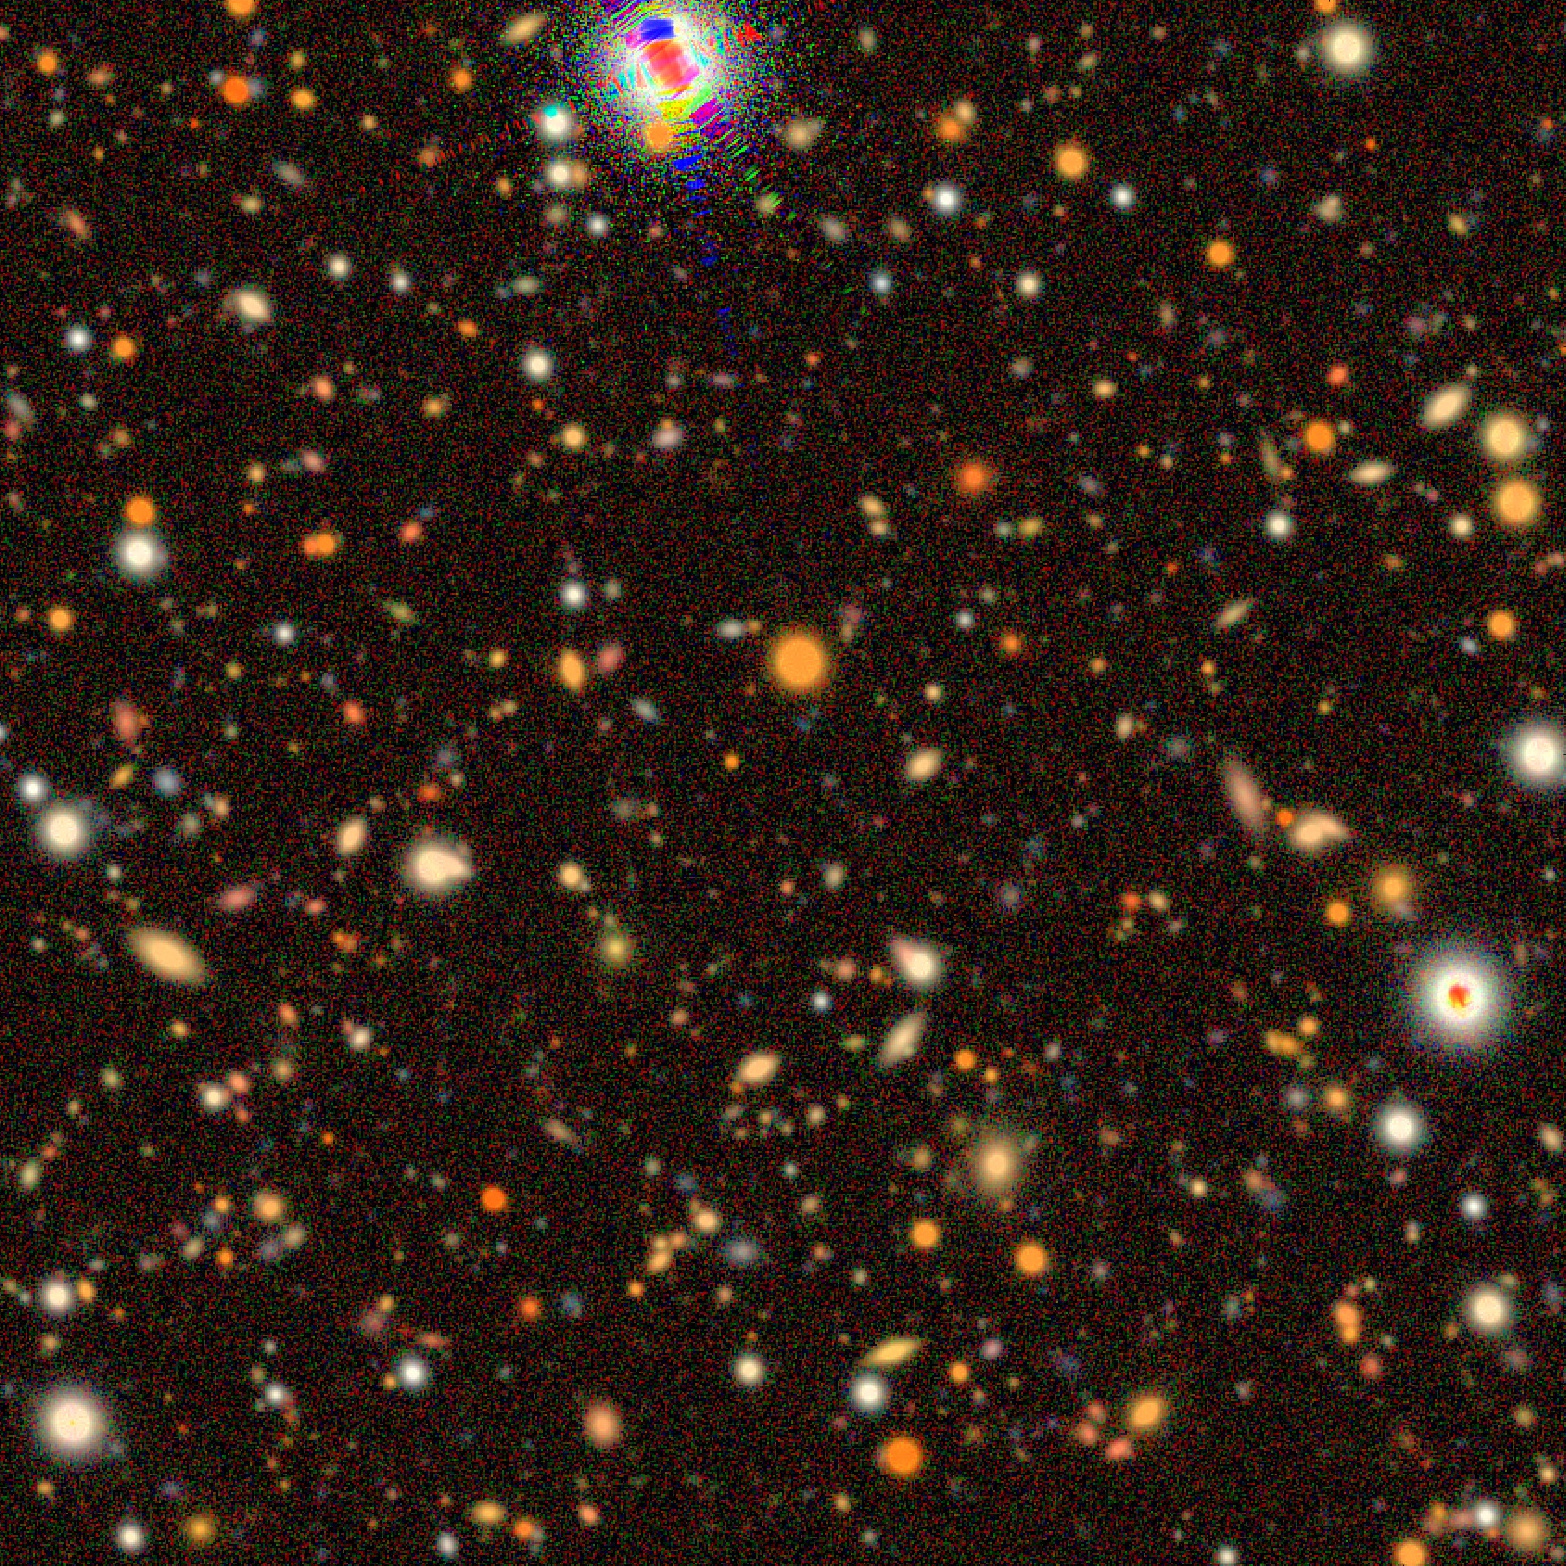
\includegraphics[width=\columnwidth]{example-image.jpg}
    \caption{
        Example simulated image. \esstodo{caption}
    }
\end{figure}
\begin{figure}
    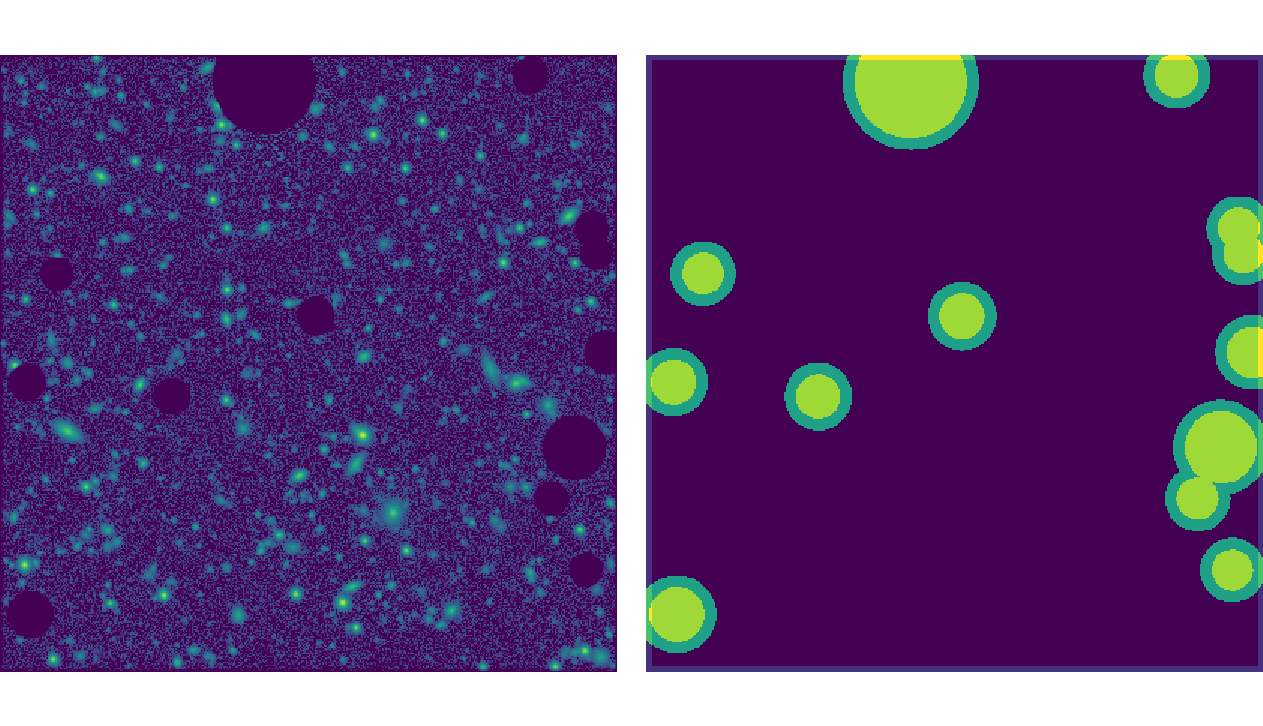
\includegraphics[width=\columnwidth]{example-masked-image.pdf}
    \caption{
        Example masked images. \esstodo{caption}
    }
\end{figure}



\section{Image and PSF Coaddition} \label{sec:coadding}

For coaddition, we used the package \texttt{descwl\_coadd} version
0.3.0\footnote{\url{https://github.com/LSSTDESC/descwl_coadd}}.  This code uses
\dm\ algorithms for warping images onto the coadd pixel grid, in particular the
\texttt{AccumulatorMeanStack} from \texttt{lsst.meas.algorithms} sub package.
We used an inverse variance weighting, based on the noise in the image.

Before warping, we interpolated artifacts such as cosmic rays, bad columns, and
saturated pixels.  The interpolation and warping modifies the noise properties
of the image.  Thus, for accurate \mcal\ noise corrections (see \S
\ref{sec:sim:noiseimages}) we must also run the noise image through the same
procedures.  Rather than use the \dm\ codes, we performed all interpolation of
artifacts and saturated regions using the \texttt{CloughTocher2DInterpolator}
from the scipy software
package\footnote{\url{https://docs.scipy.org/doc/scipy/reference/generated/scipy.interpolate.CloughTocher2DInterpolator.html}}.
We used this interpolation because the \dm\ cosmic ray interpolation available
at the time of writing is intertwined with the detection of cosmic rays, so
cannot be run on the noise image.

Using the same code, we also created PSF coadded images.  For each input image,
we generated an image of the PSF at the location of the coadd center, including
any sub-pixel offsets between the pixel grids, so the PSF images where
generally not centered.  We then warped on these images using the same weights
as the image data.  This off-centering and warping is important so that the PSF
includes the same small amount of smearing present in the image interpolation.
Not including this offset results in percent level multiplicative shear biases
(TODO cite bob's paper).  Note \dm\ provides a PSF coadding code, but at the
time of writing it did not perform sub-pixel offsets, so was unsuitable for
our purposes.

The resulting coadd and PSF coadd data were stored in a new \calexp\ data
structure for use in \mdet.

\section{Metadetection} \label{sec:mdet}

For shear inference we used the \mdet\ method presented in \cite{mdet20}.
\Mdet\ is an extension of the \mcal\ method
\citep{HuffMcal2017,SheldonMcal2017} to include the object identification
stage. We call this ``detection'', meaning specifically object identification
rather than detection of pixels with significant signal.  \Mdet\ mitigates
biases due to the shear-dependent nature of the detection processing in finite
resolution images, which are expected to be a few percent for LSST
\citep{mdet20}.

Briefly, with \mdet\ we assume that the true applied, two-component shear
$\boldsymbol{\gamma}$ is small, so that a measured ellipticity $\boldsymbol{e}$
of a galaxy is linear in the shear:
\begin{eqnarray} \label{eq:response}
\boldsymbol{e} & \approx & \left.\boldsymbol{e}\right|_{\gamma=0} +
                           \left.\frac{\partial \boldsymbol{e}}{\partial\boldsymbol\gamma}\right|_{\gamma=0} \boldsymbol\gamma +
                           O(\boldsymbol\gamma^2)\nonumber\\
               & \equiv  & \left.\boldsymbol{e}\right|_{\gamma=0} +
                           \boldsymbol{R} \boldsymbol\gamma +
                           O(\boldsymbol\gamma^2)
\end{eqnarray}
Here, the matrix $\boldsymbol{R}$ represents the linear response of the
measurement to an applied shear. It can be written component wise as
$R_{ij}=\partial e_i /\partial \gamma_j$, with $i$ and
$j$ taking all combinations of the two shear components.  For ellipticity
measurements we use weighted moments (see \S \ref{sec:mdet:meas}).

We use a finite difference to estimate $\boldsymbol{R}$.  The image is
deconvolved by the PSF, sheared, and reconvolved with a round kernel.  This
process is repeated for a small positive and negative shear, and a finite
difference response term is formed
\begin{equation}
R_{ij} \approx \frac{e_i^{+} - e_i^{-}}{\Delta\gamma_j}\ .
\end{equation}
where $e_i^{+}$ is measured on the positively sheared image and $e_i^{-}$ is
measured on the negatively sheared image.

As mentioned in \S \ref{sec:sim:noiseimages}, the deconvolve, shear, reconvolve
process produces a spurious shear response that we correct by adding a noise
image run through the same process but with orthogonal shear.

The responses too noisy to be applied to individual ellipticity measurements.
We instead average the shapes and responses in equation \ref{eq:response} to
recover a mean shear \vecg
\begin{eqnarray} \label{eq:shearmeas}
    \left< \boldsymbol{R} \right> &=& \left< \frac{\partial \boldsymbol{e} }{\partial \boldsymbol{\gamma} } \biggr\rvert_{\gamma=0} \right>, \nonumber \\
    \langle R_{ij}\rangle &=& \left< \frac{e_i^{+} - e_i^{-}}{\Delta\gamma_j} \right>, \nonumber \\
    \langle \vecg \rangle & \approx & \langle \boldsymbol{R}\rangle^{-1}\langle\boldsymbol{e}\rangle.
\end{eqnarray}

However, this process is incomplete:  the detection phase also depends on
shear.  We can incorporate detection by running object detection on the image
as well as the sheared images independently and producing the averages from
separate catalogs.  Moving the derivative outside of the average, we find
\begin{eqnarray} \label{eq:fullR}
    \left< \boldsymbol{R} \right> &=& \frac{\partial \left< \boldsymbol{e} \right> }{\partial \boldsymbol{\gamma} } \biggr\rvert_{\gamma=0},  \nonumber \\
    \langle R_{ij}\rangle &=& \frac{\langle e_i^{+}\rangle - \langle e_i^{-}\rangle}{\Delta\gamma_j} \nonumber \\
\end{eqnarray}
where now the averages for $e_i^{+/-}$ are for object catalogs found on the
respective ${+/-}$ sheared image.

For \mdet, we used the package \texttt{metadetect} version
0.6.1b\footnote{\url{https://github.com/esheldon/mdetadetect}}.  In the following subsections
we will describe parts of this process in more detail.

\subsection{Creation of Sheared Images} \label{sec:mdet:sheared}

For this work we used \dm\ data structures to represent image data (see \S
\ref{sec:sim}).  We adapted the \mcal\ implementation for creating sheared
images from the \texttt{ngmix}
package\footnote{\url{https://github.com/esheldon/ngmix}} to use these data
structures.  The new code is part of the \texttt{metadetect} software package.


\subsection{Detection and Deblending} \label{sec:mdet:detect}

We used the \dm\ algorithm for detection (TODO cite Jims paper).  We ran with
the default settings at the time of writing, which retains sources with a
$S/N \gtrsim 5$ calculated from a PSF template flux measurement.

Deblending was performed during the object detection phase as part of the
process of finding sub-peaks, but we did not use the deblender to remove the
light of neighboring objects when measuring object properties (see \S
\ref{sec:mdet:meas}).  We found that using the models to remove neighbor light
resulted in shear biases of order ten percent.

We did limited testing with the Scarlet (TODO cite) deblender, which has
recently received support in the \dm\ software stack. Scarlet performed better
in the tests we performed, showing a bias of $< 1$\%, but due to the high
computational cost of the deblender, we did not gather enough statistics to
perform more precise tests.

As we will show in \S \ref{sec:results}, measuring shapes without deblending
the light of neighbors caused no detectable bias.  However, deblending will
presumably improve the performance of other critical algorithms such as 
redshift determination.  We will explore deblending more in future work.

\subsection{Object Measurement} \label{sec:mdet:meas}

We used version v2.0.6 of the \ngmix\ package to measure weighted moments for
each detected object. The weight function was a fixed, circular, Gaussian $G(x,
y)$ with full width at half maximum of 1.2 arcseconds.  We recorded the flux,
S/N, second moments, and ellipticity derived from the second moments:
\begin{eqnarray} \label{eq:moments}
    F &=& \sum G(x, y) I(x, y) \\
    \sigma^2(F) &=& \sum \sigma^2(I(x, y)) \\
    T &=& \sum G(x, y) I(x, y) ~ (x^2 + y^2) \\
    M_1 &=& \sum G(x, y) I(x, y) ~ (x^2 - y^2) \\
    M_2 &=& \sum G(x, y) I(x, y) ~ 2 x y \\
    e_1 &=& M_1 / T \\
    e_2 &=& M_2 / T \\
    S/N &=& F / \sigma(F)
\end{eqnarray}
where $I(x, y)$ is the intensity of the image, and $\sigma^2(I(x, y))$ is the
noise variance. The sums run over all pixels in a 48x48 postage stamp image
extracted around the object of interest.  The $x$ and $y$ coordinates are
relative to the center found during detection.  Note in practice we weight each
pixel in the sum by the inverse noise variance. However, the noise variance is
nearly constant across the coadd so this is only relevant for masked, zero
weight pixels.  Note $T$ is the basic measure of size we use for applying
cuts to the object size.

We also record the moments of the coadded PSF for use in object selection (see
\S \ref{sec:results:full}).


\section{Running the Simulation and Metadetection} \label{sec:timing}

We used the ``wrapper'' package \texttt{mdet-lsst-sim} version
0.3.0\footnote{\url{https://github.com/esheldon/mdet-lsst-sim}} to run the
simulation, coaddition and \mdet, and to organize, submit and collate large
runs on computing clusters.

In all cases we used a constant shear, with possible random orientations for
each simulated scene (see \S \ref{sec:sim:shears}).  We simulated each scene
with equal but opposite shears in order to implement the noise canceling method
of \citep{pujol2019}.  For randomized shear directions, the shape measurements
from different scenes where placed in a common reference frame before averaging
to get a mean shear.

We estimated the uncertainty in the averaged shear measurements using a
jackknife technique, with chunks defined as a few tens to hundreds of scenes.

\section{Results} \label{sec:results}

In this section we present the results for various simulation and analysis
configurations.

We consider our ``base'' simulation to be one with fixed size, high S/N, round
galaxies on a grid layout, which provides the highest signal-to-noise ratio for
the shear recovery. From the results in \citet{mdet20}, we expect a small bias
in this configuration due to higher order shear effects (see \S
\ref{sec:results:base}).

We performed shear recovery with each additional feature separately in order to
isolate the cause of potential biases.  We found a bias only in the case of
extreme spatial PSF variation with few simulated epochs (see \S
\ref{sec:results:psfvar}).  We present results with all simulated features in
\S \ref{sec:results:cells}.

To characterize the bias, we assume a simple linear model \citep[see,
e.g.,][]{heymans2006} for estimating a bias in the recovered shear
\begin{equation} \label{eq:m}
\vecg = \vecc + (1 + \vecm) \vecgam
\end{equation}
where \vecg\ is the inferred shear, measured using equation \ref{eq:shearmeas},
\vecgam\ is the true shear, \vecc\ is the additive bias, and \vecm\ is the
multiplicative bias. We found \vecc\ was consistent with zero in all tests, so
in what follows we only report \vecm.

\esstodo{Establish higher order shear effects with grid/simple.  Demonstrate PS
PSF fine for expected variation, more epochs needed for higher variation (10).
Show full stars sim with cells.  Define m and c}

\subsection{Baseline Results for Fixed Galaxies on a Grid} \label{sec:results:base}

In order to establish a baseline for the bias due to higher order shear
effects, we ran a simulation with fixed, round exponential, S/N $= 10,000$,
half light radius 0.5 arcsecond galaxies placed in the grid layout (see
sections \ref{sec:sim:galaxies} and \ref{sec:sim:layouts}) with image dithers
and rotations.  In order to make the test as efficient as possible, we used
only the $i$ band with a single image ``epoch'', but with approximately the
full expected LSST 10 year depth in the combined $r, i, z$ bands.  We used a
fixed Moffat PSF\citep{Moffat1969} with FWHM=0.8.  We expect a bias $m$ of a
few parts in ten thousand for this sim \citep{SheldonMcal2017}.  We found a
bias of $4.2\times 10^{-4} < m < 4.3\times 10^{-4}$ (99.7\% confidence),
consistent with our expectations. 

We reran this simulation after all major code updates as a kind of extended
unit test to look for bugs and regressions.

\subsection{PSF Variation} \label{sec:results:psfvar}

\mdet\ requires artificially sheared versions of each coadd image (see \S
\ref{sec:mdet}).  This process involves deconvolving the image by the PSF (see
\S \ref{sec:mdet}).  This would require a spatially dependent convolution
kernel when the PSF has spatial variations.  However, due to the camera
rotations, and large number of images used to make the coadd, we expect most of
this PSF variation to be averaged down.  Thus the single coadded PSF that we
generate at the coadd center (see \S \ref{sec:sim:psfs}) may be sufficient.

We ran the same grid simulation from \S \ref{sec:results:base} with the
spatially varying PSF presented in \S \ref{sec:sim:psfs}. We used the $r, i, z$
bands but with a single image epoch per band, with rotations and dithers. We
did not see any increase in the bias.   We interpret this result to indicate
that the PSF variation is small enough that our single coadded PSF is
sufficient, even with a single image per band.

We also ran with the same simulation configuration, but with ten times the
expected PSF variation. In this case, for a single, full depth image per band,
we found a small increase in the bias $m \sim 0.0016$.  However, after
increasing the number of simulated epochs per band to ten, we found this extra
bias was removed.  We interpret this to mean that more epochs are required to
cancel out very large PSFs.  LSST will take hundreds of images in each band
(\esstodo{cite}), so we do no expect PSF variation to be a significant source
of bias.

For the remaining tests in this paper we use the spatially variable PSF with
expected variation level.

\subsection{Results with Additional Simulation Features} \label{sec:results:more}

We ran the simulation with realistic galaxies, random layout, and image
artifacts, and background subtraction errors, as listed in \S \ref{sec:sim}.
For the realistic galaxy configuration, adopted a basic set of cuts
\begin{eqnarray}
    \mathrm{S/N} & > & 10 \\
    T/T_{PSF} & > & 1.2
\end{eqnarray}
where $T$ is the Gaussian weighted square size of the object,
as defined in equation \ref{eq:moments}, and $T_{PSF}$ is the corresponding
value for the PSF.

We turned on each feature separately in order to isolate possible biases.  In
no case did we find additional bias in the shear recovery.  Nor did we find
any bias with alternative cuts on S/N and size ratio $T/T_{PSF}$.

\subsection{Results with Stars} \label{sec:results:full}

We included simulated stars as described in \S \ref{sec:sim:stars}.  In figure
\ref{fig:stardens} we show the multiplicative bias as a function of maximum
stellar density and various cut on masked fraction.  \esstodo{figure with more
varied cuts on mfrac}

\begin{figure}
	\includegraphics[width=\columnwidth]{{run-riz-drcbWsBP-cells-s2n10-100-Tratio1.2-sdens}.pdf}
	\caption{\esstodo{caption}} \label{fig:stardens}
\end{figure}

\subsection{Results with Overlapping Coadd Cells} \label{sec:results:cells}

We ran a modification of the base simulation as described in \S
\ref{sec:results:base} with a randomized position layout and overlapping cells
as described in \S \ref{sec:sim:cells}.  Because the cells overlap, the catalog
created for each coadd must be trimmed to a unique region.  Shear changes the
locations of objects, so this trimming introduces a shear dependent selection
effect.

In the case where the true simulated shear aligns with the artificially applied
shear used to create the \mcal\ images, we found that \mdet\ correctly
calibrated this effect.  However, when using randomized shear orientations (see
\S \ref{sec:sim:shears}), we found the multiplicative bias $m$ was reduced
below the expected bias due to higher order shear effects by about $-0.0004$.
We interpret this to mean that the artificial shearing slightly over-predicts
the selection effect when it is not perfectly aligned with the true shear.
This bias is smaller than LSST requirements.  However, we speculate that using
artificial shears with random orientations could mitigate this effect.   We may
explore this in more in a future work.

\subsection{Shear Sensitivity and Effective Density} \label{sec:results:effdens}

The uncertainties presented thus far are artificially reduced due to the noise
cancelling effect (see \S  \label{sec:timing}).  In order to estimate the noise
we expect for LSST, we can use the measurements for one of the two paired
images.

For the results shown in \S \ref{sec:results:full}, we simulated approximately
31,000 square degrees of images.  We converted the measured variance to an
effective density using a simple formula
\begin{equation} \label{eq:neff}
   n = \frac{\sigma^2_{SN}}{R^2 \mathrm{A} \sigma^2_{\gamma}.
\end{equation}
In equation \ref{eq:neff}, $R$ is the scalar response from averaging the
diagonal components of the response matrix, $\sigma^2_{SN}$ is the shape noise
for our catalog, about \esstodo{get}, $\sigma^2_{\gamma}$ is the uncertainty in
the recovered shear without noise cancellation, and A is the area simulated
area.

\section{Summary} \label{sec:summary}

\esstodo{}

% 
\begin{table}
\centering
\begin{threeparttable}
      \caption{
      nostack: the LSST DM stack was not used; d: dithers; r: rotations; c: cosmic rays;
      b: bad columns; R: realistic galaxy properties and noise; v: variable pixel scale
      and WCS shear; p: psf $g_2 = 0.02$; RIZ: $r, i$ and $z$ bands used; LD: large dithers;
      VP: spatially variable moffat PSF.
      }
 \label{tab:shearmeas}

  \begin{tabular}{lcc}
    \hline
    \noalign{\vskip 1mm}
    Simulation & m (99.7\% conf.) & c (99.7\% conf.) \\
     &  $[10^{-3}]$ & $[10^{-5}]$ \\
    \noalign{\vskip 1mm}
    \hline
    \noalign{\vskip 1mm}
        nostack & -0.2 $< m_1 <$ 1.1 & -\\
        d & -1.0 $< m_1 <$ 0.6 & -\\
        dr & -0.6 $< m_1 <$ 1.0 & -\\
        drc & -0.2 $< m_1 <$ 1.2 & -\\
        drcb & -0.9 $< m_1 <$ 0.6 & -\\
        drcbR & -0.9 $< m_1 <$ 0.7 & -\\
        drcbv & -0.9 $< m_1 <$ 0.7 & -\\
        drcbvp & -0.9 $< m_1 <$ 0.7 & $-1.8 < c_2 < 1.2$\\
        drcbvpRIZ & -0.5 $< m_1 <$ 0.6 & $-1.5 < c_2 < 1.4$\\
        drcbvpLD & -0.8 $< m_1 <$ 0.9 & $-1.7 < c_2 < 1.5$\\
        drcbvRIZVP & -0.6 $< m_1 <$ 1.0 & $-1.8 < c_2 < 1.3$\\

    \noalign{\vskip 1mm}
    \hline
  \end{tabular}

    \end{threeparttable}
\end{table}



% \begin{figure}
%     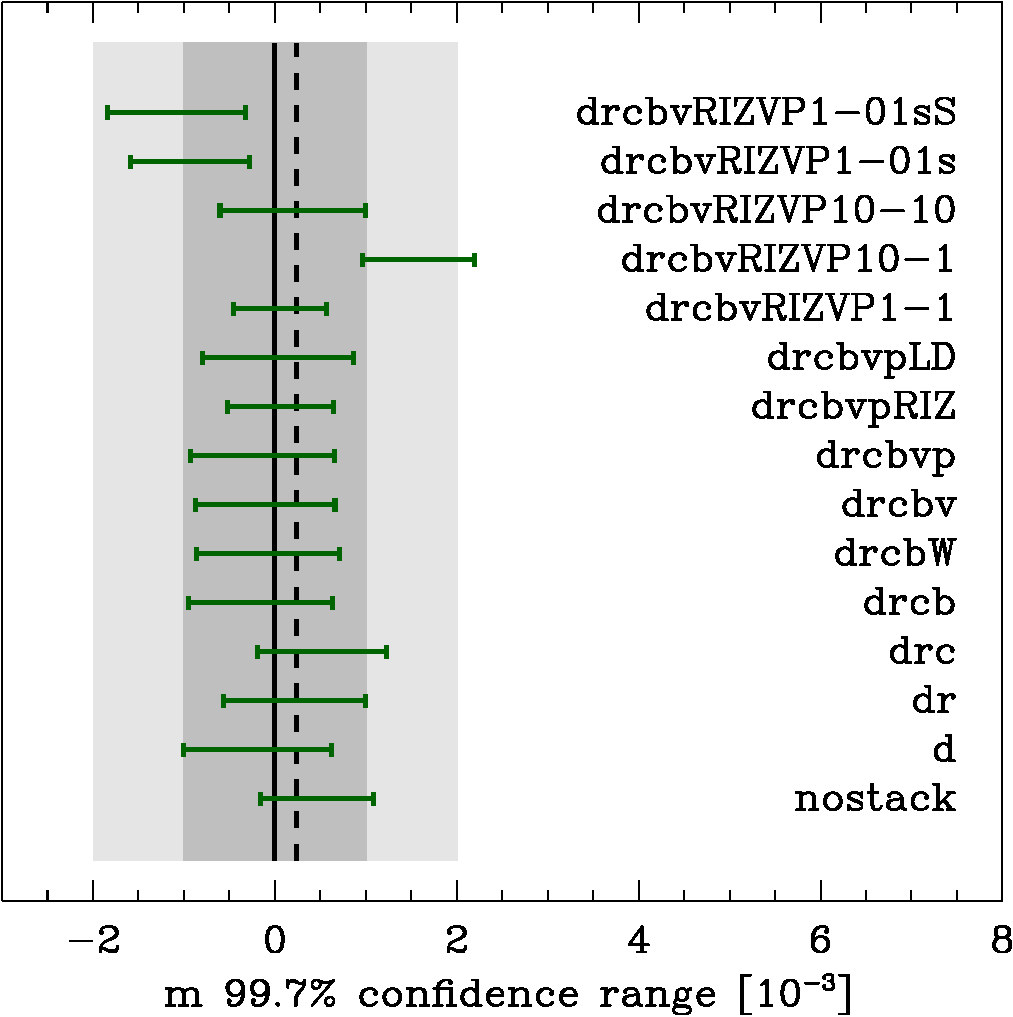
\includegraphics[width=\columnwidth]{code/mvals.pdf}
%     \caption{99.7\% confidence range for the multiplicative bias $m$ in
%      various simulations.  The light gray region represents the total
%      error budget for LSST, the dark gray region represents our target.
%      The dashed line is the expected bias due to second order shear effects.  Each
%      point represents the $m$ value measured in a particular simulation.  To the right
%      of each point is a code representing the simulation features used, which are
%      nostack: the LSST DM stack was not used; d: dithers; r: rotations; c: cosmic rays;
%      b: bad columns; W: realistic galaxy properties and noise using
%       the \descwl\ package; v: variable pixel scale
%      and WCS shear; p: psf $g_2 = 0.02$; RIZ: $r, i$ and $z$ bands used; LD: large dithers;
%      VPX-Y: spatially variable moffat PSF with X times the expected variation for LSST,
%      and Y epochs per band;  s: stars included at 2/sq arcminute, S: star masks and bleeds
%      included.
%     }
% \end{figure}

% \begin{figure}
%     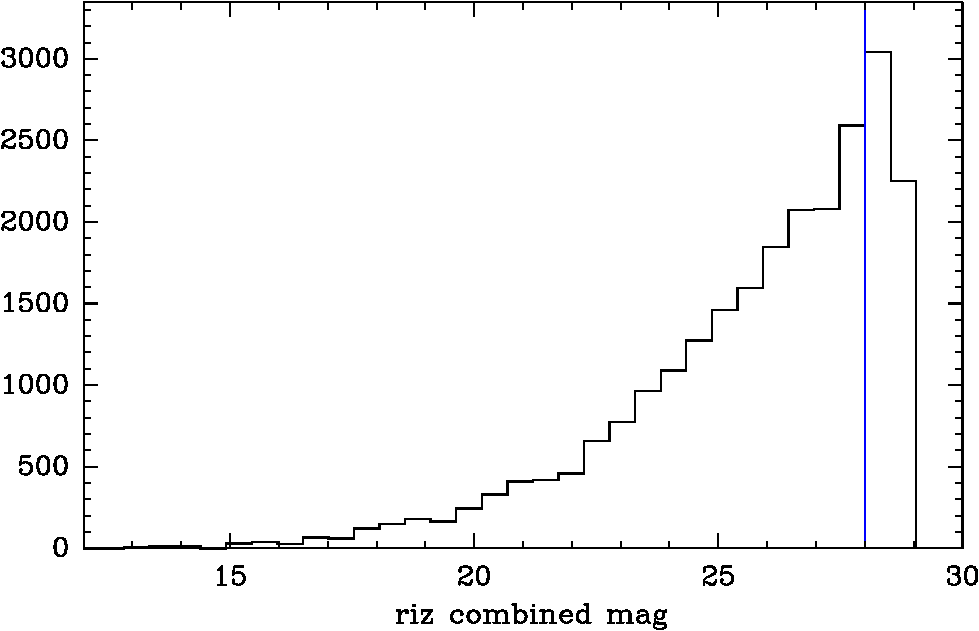
\includegraphics[width=\columnwidth]{mag-hist.pdf}
%     \caption{
%         Star magnitudes measured in simulated $r+i+z$ combined coadds.  The
%         $r-band$ magnitude limit for the input star sample is shown as a
%         vertical line at 28.  The detection in the combined image is
%         somewhat deeper.
%     }
% \end{figure}


% \begin{figure}
%     \centering
% \begin{tikzpicture}
%     \begin{groupplot}[
%         legend style={draw=none},
%         group style={group size=1 by 2, vertical sep=0.3cm},
%         xmin=0.0,
%         xmax=110.0,
%         width=0.9\columnwidth,
%         height=0.6\columnwidth,
%         minor tick num=3,
%         axis on top
%     ]
%     \nextgroupplot[
%         ylabel={$m/10^{-3}$},ymin=-2,xticklabels={,,},
%         ymin=-2, ymax=2
%     ]
%
% 	\addplot+[name path=A,gray!20,no markers] coordinates {
%         (0.0,-1)
%         (110.0,-1)
%     };
%     \addplot+[name path=B,gray!20,no markers] coordinates {
%         (0.0,1)
%         (110.0,1)
%     };
%
%     \addplot+[gray!20] fill between[of=A and B];
% 	\addplot+[black!80,no markers] coordinates {
%         (0.0,0.0)
%         (110.0,0.0)
%     };
%
% 	% \addplot+[
%     %     brown!60!black,mark=otimes*, mark options={fill=brown!40},
%     %     error bars/.cd,y dir=both,y explicit] table[x index=0, y index=1, y error index=2
%     % ] {code/m-vs-star-density.txt};
%
% 	\addplot+[
%         brown!60!black,mark=otimes*, solid, mark options={fill=brown!40},
%         error bars/.cd,y dir=both,y explicit] table[x index=0, y index=1, y error index=2
%     ] {code/m-vs-star-density-s2n10.txt};
%
% 	\addplot+[
%         teal!60!black,mark=triangle*, solid, mark options={fill=teal!40},
%         error bars/.cd,y dir=both,y explicit] table[x index=0, y index=1, y error index=2
%     ] {code/m-vs-star-density-s2n15.txt};
%
% 	\addplot+[
%         red!60!black,mark=diamond*, solid, mark options={fill=red!40},
%         error bars/.cd,y dir=both,y explicit] table[x index=0, y index=1, y error index=2
%     ] {code/m-vs-star-density-s2n20.txt};
%
% 	\addplot+[
%         blue!60!black,mark=square*, solid, mark options={fill=blue!40},
%         error bars/.cd,y dir=both,y explicit] table[x index=0, y index=1, y error index=2
%     ] {code/m-vs-star-density-s2n25.txt};
%
% 	\addplot+[
%         brown!60!black,mark=oplus*, solid, mark options={fill=yellow!40},
%         error bars/.cd,y dir=both,y explicit] table[x index=0, y index=1, y error index=2
%     ] {code/m-vs-star-density-s2n30.txt};
%
%
%
%     % \nextgroupplot[
%     %     ymin=0.93,
%     %     xlabel=Stellar Density Cut {[\#/sq arcmin]},ylabel={$\sigma_m/\sigma_m^{100}$}
%     % ]
%
% 	% \addplot+[black!80,no markers] coordinates {
%     %     (0.0,1.0)
%     %     (110.0,1.0)
%     % };
%
%     % \addplot+[
%     %     teal!60!black,mark=triangle*, mark options={fill=teal!40},
%     %     error bars/.cd,y dir=both,y explicit] table[x index=0, y index=3
%     % ] {code/m-vs-star-density.txt};
%
%     \nextgroupplot[
%         xlabel=Stellar Density Cut {[\#/sq arcmin]},ylabel={$\sigma_m$},
%         ymin=0.6, ymax=1.1
%     ]
%
% 	\addplot+[
%         brown!60!black,mark=otimes*, solid, mark options={fill=brown!40} 
%         ] table[x index=0, y index=2,
%     ] {code/m-vs-star-density-s2n10.txt};
%     \addlegendentry{$S/N > 10$}
%
% 	\addplot+[
%         teal!60!black,mark=triangle*, solid, mark options={fill=teal!40}
%         ] table[x index=0, y index=2,
%     ] {code/m-vs-star-density-s2n15.txt};
%     \addlegendentry{$S/N > 15$}
%
% 	\addplot+[
%         red!60!black,mark=diamond*, solid, mark options={fill=red!40}
%         ] table[x index=0, y index=2,
%     ] {code/m-vs-star-density-s2n20.txt};
%     \addlegendentry{$S/N > 20$}
%
% 	\addplot+[
%         blue!60!black,mark=square*, solid, mark options={fill=blue!40}
%         ] table[x index=0, y index=2,
%     ] {code/m-vs-star-density-s2n25.txt};
%     \addlegendentry{$S/N > 25$}
%
% 	\addplot+[
%         brown!60!black,mark=oplus*, solid, mark options={fill=yellow!40}
%         ] table[x index=0, y index=2,
%     ] {code/m-vs-star-density-s2n30.txt};
%     \addlegendentry{$S/N > 30$}
%
%
%     \end{groupplot}
% \end{tikzpicture}
%
%     \caption{ Metadetection performance as a function of maximum stellar
%     density and for different object S/N thresholds.  Simulations were run with
%     the expected stellar density distribution for the full LSST 18,000 square
%     degree survey, with a maximum allowed value of 100/sq. arcminute.  Stars
%     bright enough to saturate were not included.  Top panel:  the
%     multiplicative bias $m$ as a function of the stellar density cut and S/N
%     threshold.  Objects with small measured size $T/T_{\mathrm{PSF}} < 1.2$
%     were removed, where $T = \langle x^2 \rangle + \langle y^2 \rangle$ is the
%     estimated psf convolved size of the object.  Bottom panel: the uncertainty
%     on the mean shear as a function of the stellar density cut, for different
%     S/N thresholds.  Note that many lensing probes are dominated by cosmic
%     variance, which is not included in these uncertainties.  }
%
% \end{figure}
%
%
% \begin{figure}
%     \centering
% \begin{tikzpicture}
%     \begin{axis}[
%         legend style={draw=none,at={(0.97,0.5)},anchor=east},
%         ylabel={$m/10^{-3}$},
%         xlabel={Stellar Density $[\#/sq. arcmin]$},
%         xmin=-5.0,
%         xmax=190.0,
%         ymin=-8,
%         ymax=8,
%         width=0.9\columnwidth,
%         height=0.6\columnwidth,
%         minor tick num=4,
%         axis on top
%     ]
%
% 	\addplot+[name path=A,gray!20,no markers, forget plot] coordinates {
%         (0.0,-1)
%         (110.0,-1)
%     };
%     \addplot+[name path=B,gray!20,no markers, forget plot] coordinates {
%         (0.0,1)
%         (110.0,1)
%     };
%
%     \addplot+[gray!20, forget plot] fill between[of=A and B];
% 	\addplot+[black!80,no markers, forget plot] coordinates {
%         (0.0,0.0)
%         (110.0,0.0)
%     };
%
% 	\addplot+[
%         brown!60!black,mark=otimes*, solid, mark options={fill=brown!40},
%         error bars/.cd,y dir=both,y explicit] table[x index=0, y index=1, y error index=2
%     ] {code/mc-results-run-drsBMWRIZ-v1/m-vs-star-density-s2n10.txt};
%     \addlegendentry{$S/N > 10$}
%
% 	\addplot+[
%         teal!60!black,mark=triangle*, solid, mark options={fill=teal!40},
%         error bars/.cd,y dir=both,y explicit] table[x index=0, y index=1, y error index=2
%     ] {code/mc-results-run-drsBMWRIZ-v1/m-vs-star-density-s2n15.txt};
%     \addlegendentry{$S/N > 15$}
%
% 	\addplot+[
%         red!60!black,mark=diamond*, solid, mark options={fill=red!40},
%         error bars/.cd,y dir=both,y explicit] table[x index=0, y index=1, y error index=2
%     ] {code/mc-results-run-drsBMWRIZ-v1/m-vs-star-density-s2n20.txt};
%     \addlegendentry{$S/N > 20$}
%
% 	\addplot+[
%         blue!60!black,mark=square*, solid, mark options={fill=blue!40},
%         error bars/.cd,y dir=both,y explicit] table[x index=0, y index=1, y error index=2
%     ] {code/mc-results-run-drsBMWRIZ-v1/m-vs-star-density-s2n25.txt};
%     \addlegendentry{$S/N > 25$}
%
% 	\addplot+[
%         brown!60!black,mark=oplus*, solid, mark options={fill=yellow!40},
%         error bars/.cd,y dir=both,y explicit] table[x index=0, y index=1, y error index=2
%     ] {code/mc-results-run-drsBMWRIZ-v1/m-vs-star-density-s2n30.txt};
%     \addlegendentry{$S/N > 30$}
%
%
%     \end{axis}
%
% \end{tikzpicture}
%
%     \caption{ Metadetection multiplicative bias as a function of maximum
%     stellar density and for different object S/N thresholds.  Simulations were
%     run with the expected stellar density distribution for the full LSST 18,000
%     square degree survey, with a maximum allowed value of 100/sq. arcminute.
%     Stars were simulated as Moffat profiles and were allowed to saturate, with
%     simulated bleed trails.  A circular mask was used for saturates stars and
%     this area was interpolated.  Error bars are 99.7\% confidence regions.
%     Objects with small measured size $T/T_{\mathrm{PSF}} < 1.2$ were removed,
%     where $T = \langle x^2 \rangle + \langle y^2 \rangle$ is the estimated psf
%     convolved size of the object.}
%
% \end{figure}
%
%
%
%
%
% \begin{figure}
%     \centering
% \begin{tikzpicture}
%
% 	\begin{axis}[
%         legend style={draw=none},
%         xlabel=min S/N,
%         ylabel={$\sigma/\sigma_{\mathrm{no~stars}}$},
%         xmin=5.0,
%         xmax=50.0,
%         ymin=1.1,
%         ymax=1.225,
%         width=0.9\columnwidth,
%         height=0.6\columnwidth,
%         minor tick num=3,
%         axis on top
% 	]
%
% 	%\addplot+[black,no markers] coordinates {
%     %    (0.0,1.0)
%     %    (110.0,1.0)
%     %};
%
%
%         %\addplot+[brown!60!black,mark=otimes*, solid, mark options={fill=brown!40}]
%         %    table[x index=0, y index=1] {code/mc-results-6700/noise-ratio-dcut010.txt};
%         %\addlegendentry{$d < 10$}
%
%         \addplot+[teal!60!black,mark=triangle*, solid, mark options={fill=teal!40}]
%             table[x index=0, y index=1] {code/mc-results-6700/noise-ratio-dcut020.txt};
%         \addlegendentry{$d < 20$}
%
%         \addplot+[red!60!black,mark=diamond*, solid, mark options={fill=red!40}]
%             table[x index=0, y index=1] {code/mc-results-6700/noise-ratio-dcut040.txt};
%         \addlegendentry{$d < 40$}
%         \addplot+[blue!60!black,mark=square*, solid, mark options={fill=blue!40}]
%             table[x index=0, y index=1] {code/mc-results-6700/noise-ratio-dcut060.txt};
%         \addlegendentry{$d < 60$}
%         \addplot+[brown!60!black,mark=oplus*, solid, mark options={fill=yellow!40}]
%             table[x index=0, y index=1] {code/mc-results-6700/noise-ratio-dcut080.txt};
%         \addlegendentry{$d < 80$}
%         \addplot+[orange!60!black,mark=*, solid, mark options={fill=orange!40}]
%             table[x index=0, y index=1] {code/mc-results-6700/noise-ratio-dcut100.txt};
%         \addlegendentry{$d < 100$}
%
%
% 	\end{axis}
% \end{tikzpicture}
%
%     \caption{Increased noise in the recovered shear when stars are present in
%     the simulation, compared to a simulation without stars, as a function of
%     the minimum signal-to-noise ratio and maximum stellar density.  The stellar
%     density was drawn from the expected distribution for the full LSST 18,000
%     square degree survey, including regions with density as high as 100 per
%     square arcmin.  Stars were allowed to saturate, and a fixed size star mask
%     was used, but no bleed trails were present.  To select galaxies, only
%     objects with size $T/T_{\mathrm{PSF}} > 1.2$ were used, where $T = \langle
%     x^2 \rangle + \langle y^2 \rangle$ is the estimated psf convolved size of
%     the object.  The lowest absolute noise is for $S/N > 10$ and a liberal cut
%     on stellar density at $d < 60$, which also results in the smallest
%     increase in noise relative to a simulation with no stars.  Note that many
%     lensing probes are dominated by cosmic variance, which is not included in
%     these uncertainties.  }
%
% \end{figure}



\section*{Acknowledgments}

ES is supported by DOE grant DE-AC02-98CH10886, and MB is supported by DOE
grant DE-AC02-06CH11357.  RA is supported by the US Department of Energy Cosmic
Frontier program, grant DE-SC0010118.  (TODO Mike's funding)

We thank Javier Sanchez for providing the star and stellar density map for DC2,
and Jim Chiang for providing example images containing simulated stars
with bleed trails.

We thank the excellent computing staffs of the RHIC Atlas Computing Facility at
Brookhaven National Laboratory and \mattodo{how to acknowledge SLAC resources?}

\esstodo{}


%\bibliographystyle{mnras}
%\bibliography{references}
%\bibliography{apj-jour,references}
%\bibliographystyle{apj}
\bibliographystyle{aasjournal}
\bibliography{references}

\end{document}
